%*****************************************
\chapter{Implementation}\label{ch:implementation}
%*****************************************

Um die Webanwendung platformübergreifend entwickeln und auf beliebigen Systemen einsetzen zu können würde ASP.NET Core MVC als Development Framework gewählt.

\section{ASP.NET Core MVC}

Die General-Purpose-Development-Platform .NET Core wurde unter Koordination von Microsoft zusammen mit der .NET Community entwickelt und als Open Source-Projekt über GitHub \cite{dotnetcore} verfügbar gemacht. Sie bietet eine platformübergreifende Lösung zur Entwicklung und Ausführung von Anwendungsprogrammen und läuft unter Windows, macOS and Linux. ASP.NET steht für Active Server Pages .NET und ist ein Web Application Framework von Microsoft, mit dem sich dynamische Webseiten, Webanwendungen und Webservices entwickeln lassen. ASP.NET Core MVC baut auf .NET Core auf und vereint die Effektivität und Übersichtlichkeit der Model-View-Controller (MVC) Architektur \cite{freeman2016pro}. Als Entwicklungsumgebung wurde Visual Studio Code, ein kostenloser und quelloffener Texteditor, mit C\# Extension genutzt.

\subsection{Model-View-Controller}

Das Model-View-Controller Design Pattern dient der Trennung der Software in die drei Komponenten

\begin{itemize}
	\item Models, die die Daten enthalten mit denen der Nutzer arbeitet
	\item Views, die Teile des Models rendern und so das User Interface darstellen 
	\item Controllers, die eingehende Anfragen annehmen und Operationen auf dem Model durchführen sowie Views die gerendert werden sollen auswählen
\end{itemize}

Allgemein kann man sagen, dass das model die Objekte der realen Welt repräsentiert, zusammen mit den Prozessen und Regeln die das  bestimmte Einsatzgebiet der App definieren. Dies wird auch als Domain der Applikation bezeichnet und analog wird das Model auch Domain Model genannt. Die C\#-Models zusammen mit ihren Methoden bilden die Wirklichkeit auf die Applikation ab. Dabei stellen die Views zusammen mit den Controllern die Domain dem Client dar.



Dabei ist jeder Teil der MVC Architektur eigenständig und wird auch `separation of concerns' genannt. So werden die Daten im Model ausschließlich vom Model verändert, die Daten ausschließlich vom View dargestellt und user requests und input ausschließlich im Controller verarbeitet. Durch diese klare Trennung der Komponenten wird es einfacher die Application zu warten und zu erweitern. Der Zusammenhang zwischen den einzelnen Komponenten ist in Abbildung \ref{fig:mvc} dargestellt.

\begin{figure}
\centering
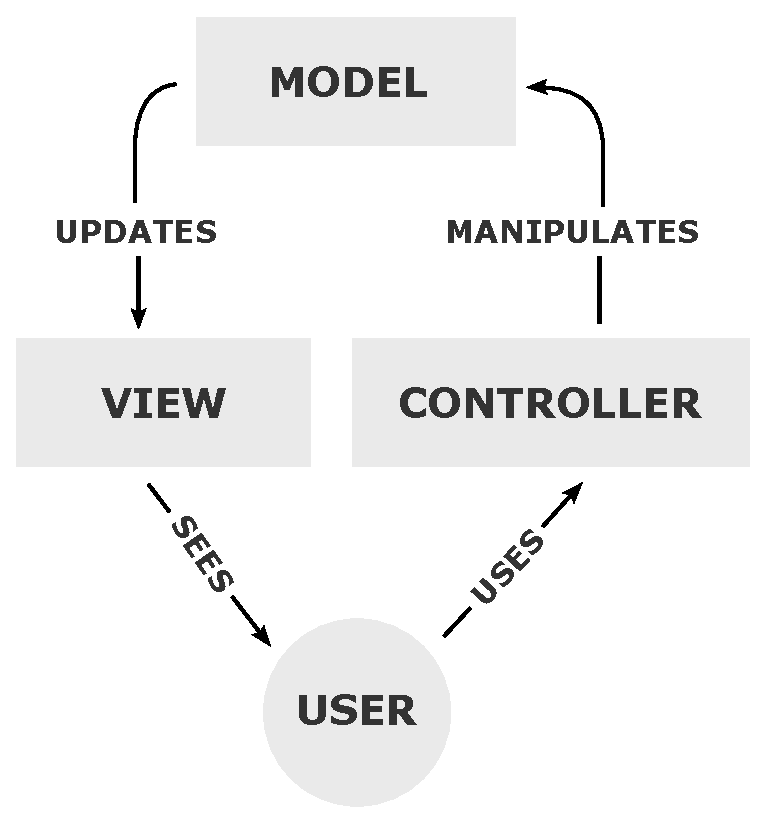
\includegraphics[width=6cm]{Figures/mvc}
\caption{Model-View-Controller}
\label{fig:mvc}
\end{figure}

 Beim MVC-Pattern werden eingehende Anfragen durch Controller behandelt. In ASP.NET Core MVC sind Controller C\#-Klassen die gewöhnlich von der integrierten MVC-Controller Basisklasse \code{Microsoft.AspNetCore.Mvc.Controller} erben. Jede \code{public}-Methode eines Controllers wird auch \emph{action method} genannt. Man kann sie aus dem Web über eine URL aufrufen und so eine Aktion ausführen. In einer Web Application geht es darum dynamischen Output zu konstruieren und darzustellen. In MVC ist der Controller dafür zuständig basierend auf dem Model Daten zu konstruieren und diese an den View weiterzugeben, welcher wiederum das HTML rendert. Wenn also eine Anfrage an die URL die mit der action method verbunden ist gesendet wird, werden die Statements in der action method ausgeführt um Operationen auf domain model anzuwenden und dann ein view auszuwählen der dem Client angezeigt wird. Dies is in Abbildung \ref{fig:mvc_http} dargestellt.
 
 
 \begin{figure}
\centering
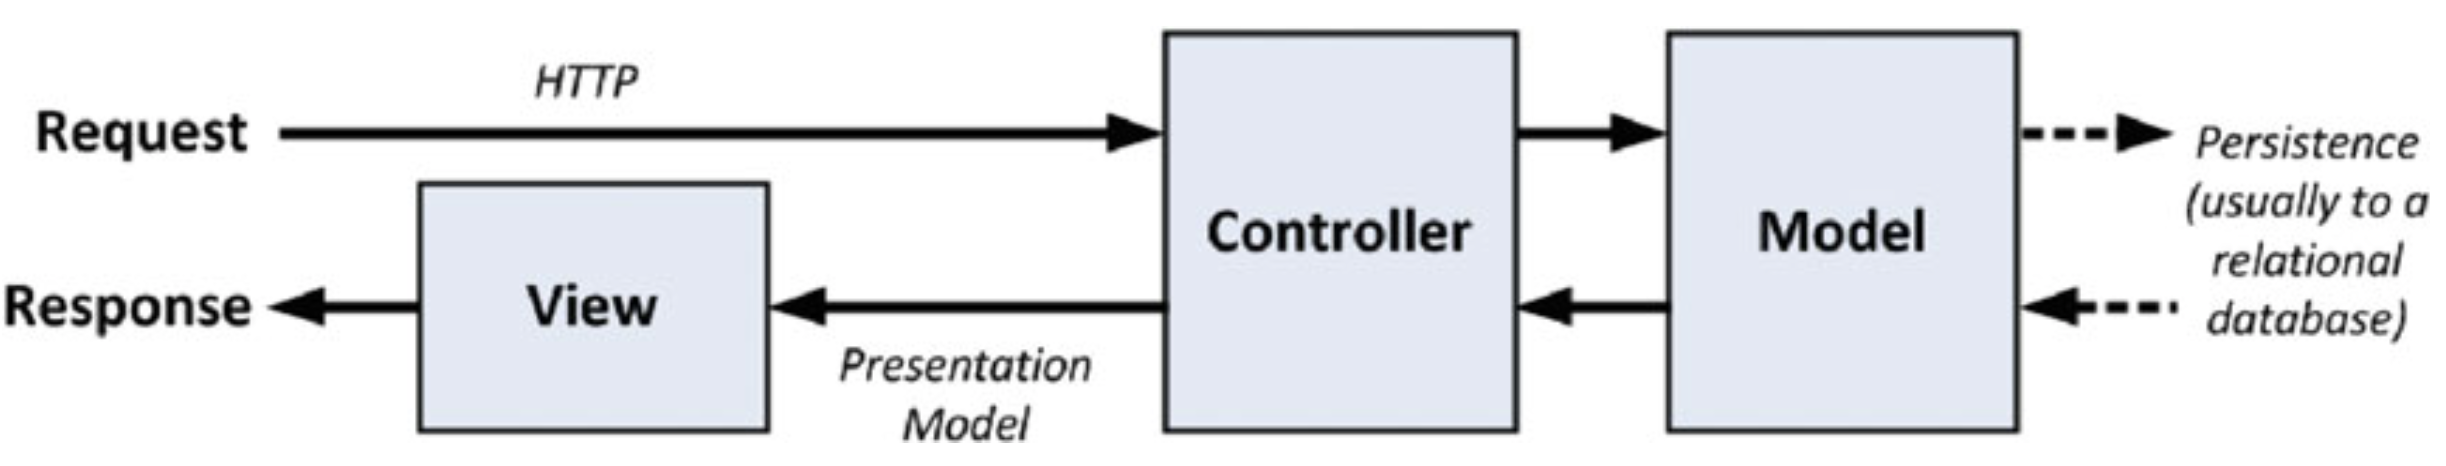
\includegraphics[width=\textwidth]{Figures/mvc_http}
\caption{HTTP request mit Model-View-Controller}
\label{fig:mvc_http}
\end{figure}
 
 
\subsection{Routes}

ASP.NET Core MVC Applications nutzen das ASP.NET routing system. Diese entschiedet welche URLs auf welchen Controller und welche Actions abgebildet werden. Eine Route ist eine Regel die darüber entscheidet wie eine Anfrage behandelt wird. Als Standardregeln für ein neues MVC Projekt sind werden beispielsweise die folgenden URLs auf die Index action des code{HomeControllers}s weitergeleitet.

\begin{itemize}

	\item /
	\item /Home
	\item /Home/Index

\end{itemize}

\noindent
Nach Konvention hat die Application einen \code{HomeController} welcher den Einstiegspunkt in die MVC Application bildet.


\subsection{Razor View Engine}

Für eine Webapplikation ist es essentiell dynamischen Inhalt zu generieren und an den Client zu senden. Die Razor View Engine ist eine ASP.NET template markup syntax die zur dynamischen Erstellung von Webseiten in C\# genutzt wird \cite{razorengine}. Dabei sind Razor views HTML templates die C\#-Logik enthalten, welche model data nutzt um dynamisch Content zu generieren. Weil Razor Expressions fast jedes gültige C\#-Statement enthalten können ist es mitunter schwierig zu entscheiden ob Logik in den View oder in den Controller gehört ohne das MVC pattern zu untergraben.

\subsection{Model Binding}

Model Binding ist ein nützliches Feature von MVC. Eingehende Daten eines HTTP-requests werden geparsed und unter Berücksichtigung der Key-Value-Pairs den Properties des jeweiligen domain models types zugewiesen. Dadurch wird das mühevolle Behandeln von HTTP requests vermieden und man kann direkt mit C\# Objekten arbeiten anstatt mit Datenpaketen die vom Browser gesendet werden.


